% !TeX root = ../artigo.tex
\section{RESULTADOS E DISCUSSÃO}
Finalizadas as configurações, tanto no sistema Unix, como em Windows, foi realizada a reinicialização dos sistemas e, a partir disso, eles foram capazes de apresentar as opções de autenticação, de acordo com os usuários cadastrados anteriormente no servidor.

\begin{figure}[ht]
    \begin{subfigure}{0.48\textwidth}
    	\centering
    	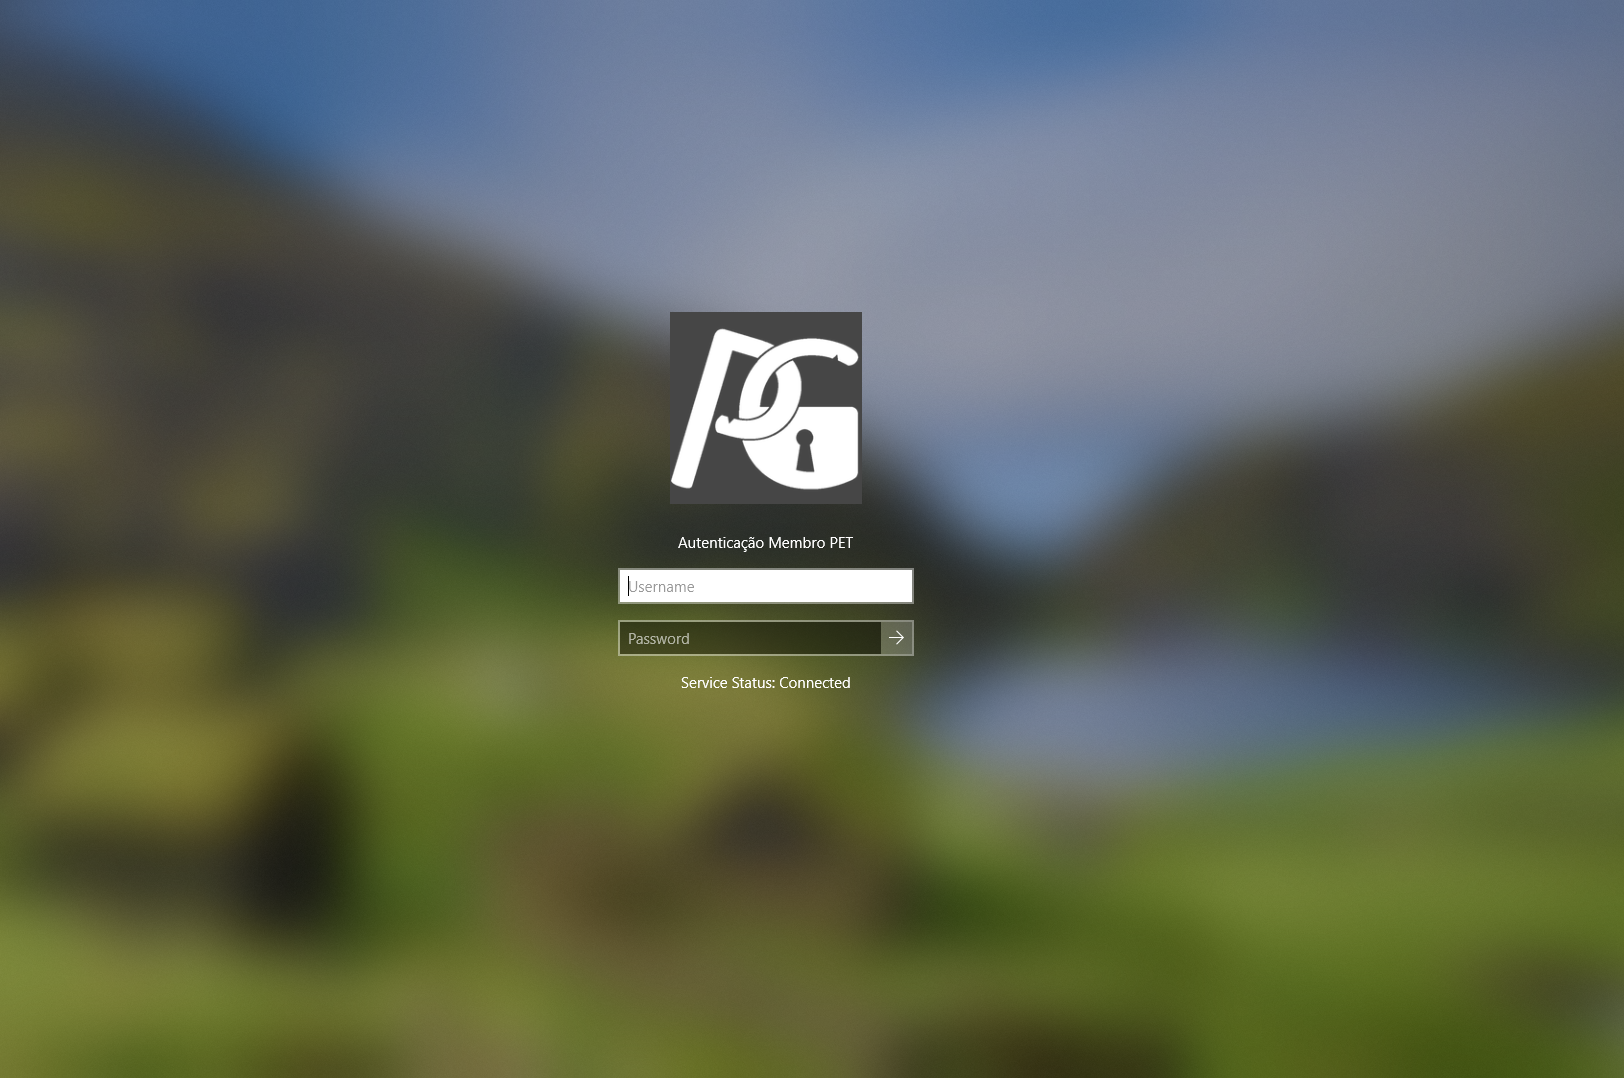
\includegraphics[height=5cm]{textuais/TelaLoginWindows.png}
    	\caption{Tela de login do Windows
    	\label{fig:telawindows}}
    \end{subfigure}%
    \hspace{0.04\textwidth} % Espaço horizontal
    \begin{subfigure}{0.48\textwidth}
    	\centering
    	
\includegraphics[height=5cm]{textuais/TelaLoginUnix.png}
    	\caption{Tela de login do Arch Linux
    	\label{fig:telaunix}}
    \end{subfigure}
    \caption{Telas de login dos sistemas}
    \label{fig:telaslogin}
\end{figure}

Ambos os sistemas foram capazes de autenticar os usuários, de acordo com as credenciais estabelecidas previamente, a medida que, qualquer alteração no servidor, é automaticamente percebida pelos clientes no momento da importação dos dados LDAP.

No momento em que o usuário se conecta em seu perfil pela primeira vez, o sistema acertadamente cria a pasta local respectiva à conta conectada, pasta essa, que apenas o próprio usuário logado
e perfis administradores possuem acesso. Além disso o sistema verifica, de acordo com as regras preestabelecidas, o grupo em que o perfil está inserido, para definir suas permissões.

Como o OpenLDAP foi desenvolvido essencialmente para sistemas Unix, seu funcionamento no Windows se limita à autenticação via perfil fixo do pGina, diferentemente do Unix, onde todos os perfis cadastrados são exibidos ao usuário no momento do acesso.

Outra limitação existente no Windows, é a de que o sistema apenas realiza a importação do DN de cada usuário, portanto, os usuários são cadastrados no sistema com o nome correspondente ao seu 'username', além disso, essa restrição impossibilita a importação de outros recursos, que possam ser adicionados ao servidor.

\subsection{Trabalhos Futuros}

Dadas as limitações do pGina, um próximo projeto interessante, seria o desenvolvimento de um sistema provedor de credenciais ainda mais completo para Windows, que seja capaz de importar todas as informações necessárias, tanto ao administrador da rede, quanto ao usuário conectado.

Outro possível trabalho, é a implementação do compartilhamento de recursos da mesma conta entre várias máquinas, esse método é viável graças ao método de autenticação centralizada adicionado aos sistemas clientes ao longo deste projeto.
